\chapter{Hardware}\label{ch:hardware}
The system presented in this paper makes use of a variety of mechanical components. This chapter will talk about mechanical challenges and our solutions that allow the construction of large-scale dynamic truss objects using 3D printed parts. It will explain the materials and methods used in creating a real-world object from a TrussFormer-designed model.\\
Furthermore, this chapter will define the techniques and hardware employed in the structures.

\section{Mechanical Components}
We can differentiate between three essential building parts for our truss objects. We call the structural components \textit{Links}. In our objects PET bottles are used as links, as they are readily available, cheap and sturdy.\\
We have two different ways of connecting links. Rigid connections are comprised of \textit{static hubs}. For dynamic connections, i.e. connections that allow movement of the structure, we use \textit{hinging hubs}.\\
Links, and static or hinging hubs are connected by purpose-designed \textit{cuffs}, which fit over the bottles' thread on one side and a connector part on the hub on the other side, as seen in Figure \ref{fig:connector} (b).

\subsection{Edges of the structure}
We opted to use 1l (big) and 0.5l (small) reusable PET bottles because they have thicker walls, providing more stability and are abundantly available. Two bottles are connected on their bottom side by a wood screw, which is inserted using a special long-necked screwdriver. This process is depicted in Figure \ref{fig:connect_bottles}. The resulting link-lengths are:
\begin{enumerate}
\item 60 cm - two big bottles
\item 53 cm - one big and one small bottle
\item 46 cm - two small bottles
\end{enumerate}

\begin{figure}[ht!]
    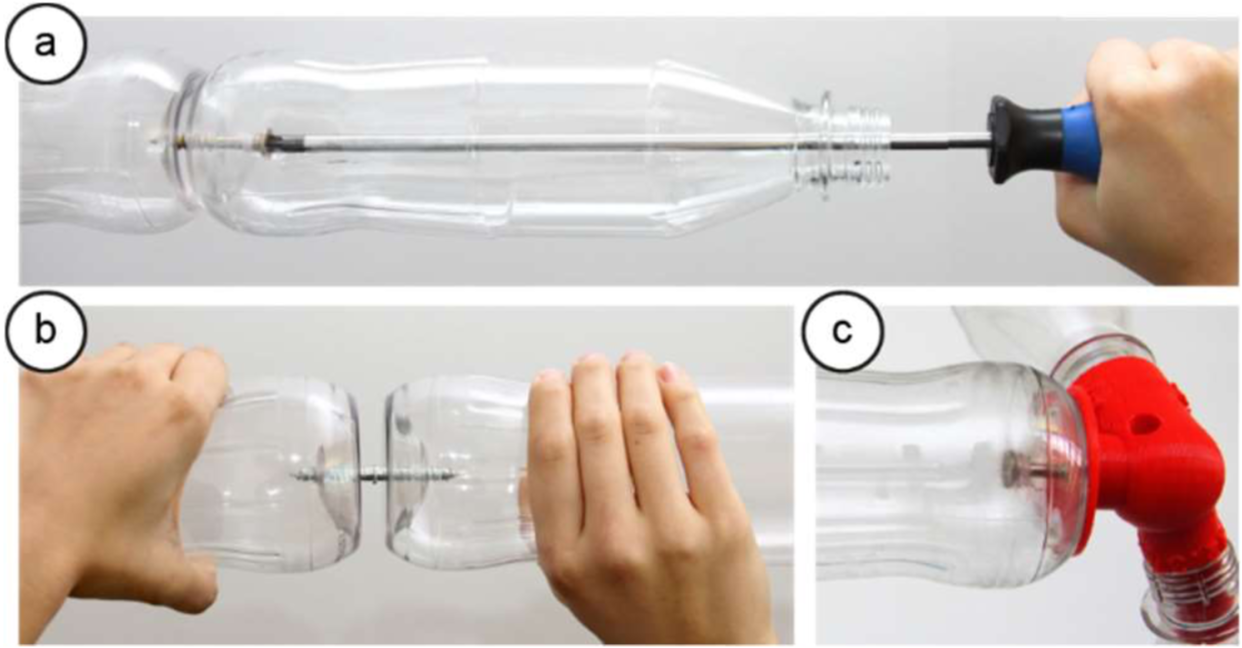
\includegraphics[width=\textwidth]{Hardware/connect_bottles.png}
    \centering
    \caption{(a) Connecting bottles with a wood screw using an extra-long screwdriver and (b) with a double-ended screw. (c) Single-bottle edges require a bottom connector}
    \label{fig:connect_bottles}
\end{figure}

\subsection{Rigid Hubs}
We call the connecting parts \textit{Hubs}. These hubs are designed to withstand loads in the range of a human weight. Earlier tests show, that the bottle links we use can withstand a compression force of around 85 kg.\\
Hubs are solid one-piece objects that can connect two or more links. They therefore have two or more regions that can hold the neck of a bottle. We call these regions \textit{connectors}. These connectors consist of a flat part, slightly wider (30 mm) than the bottle openings outer diameter (28 mm) and an extrusion in the middle, the size of its inner diameter (20 mm). The extrusion is plugged into the bottle opening, giving a snug fit and good lateral stability.\\
To prevent the bottles from slipping out, a \textit{cuff} is clipped over the connector and the bottle opening. The cuff is designed as a circular section, slightly larger than a semicircle. Its upper and lower end have different sizes: the smaller end fits over a rim on the hub connector, the larger one over an extrusion on the bottle neck. Due to its flexibility, the cuff acts like a spring, making it easy to clip over the bottle and connector, while giving enough stability once clipped on.

\begin{figure}
    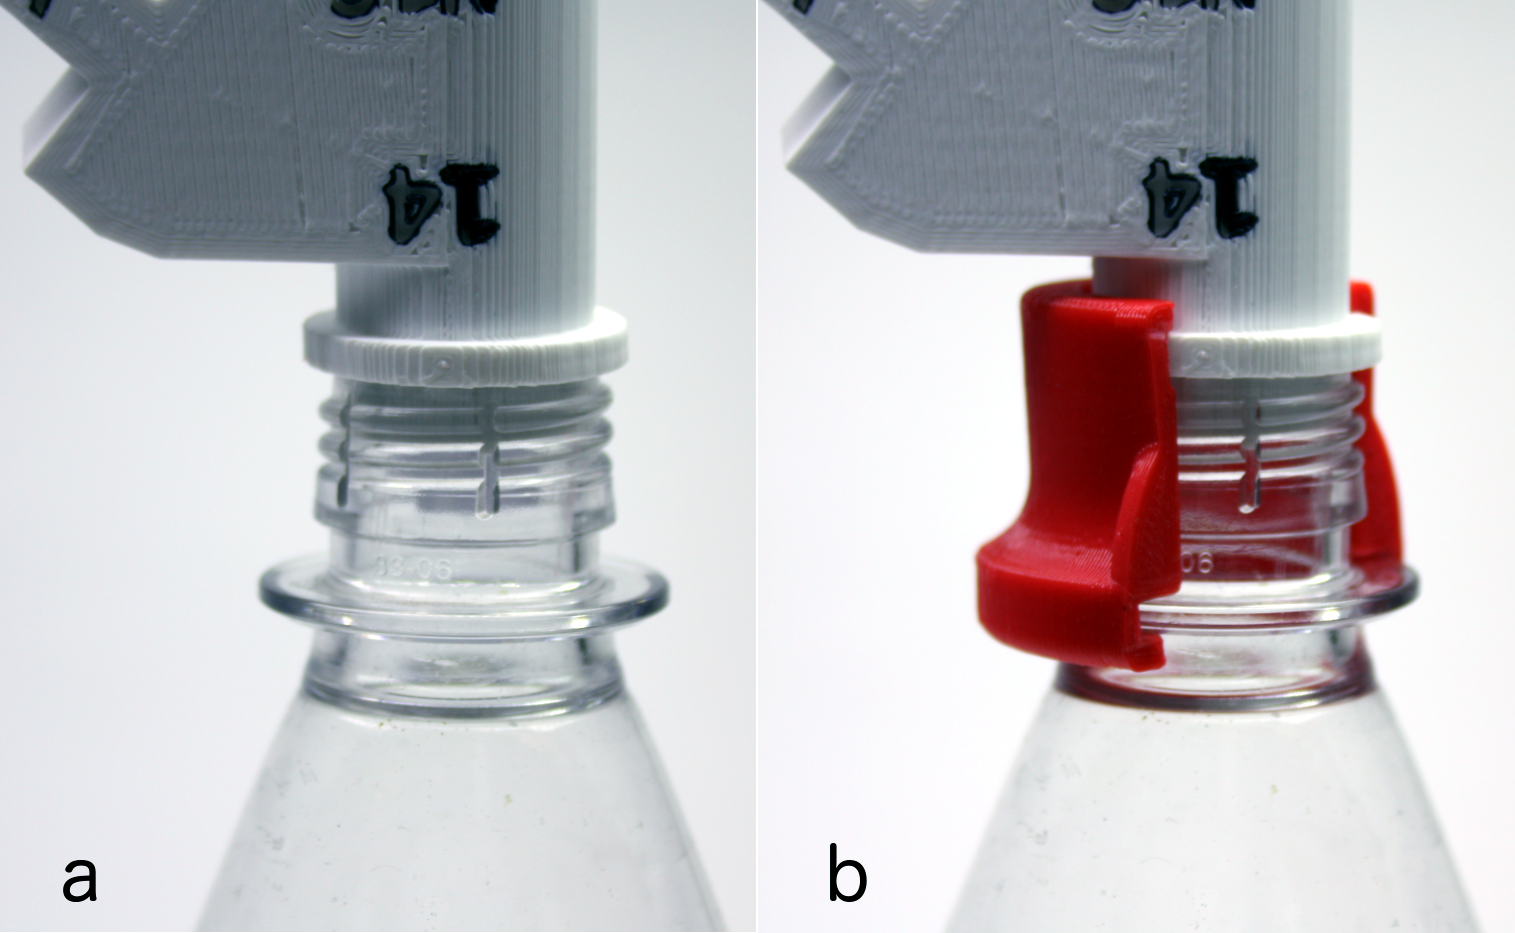
\includegraphics[width=\textwidth]{Hardware/connectors.png}
    \caption{(a) The connector is inserted into the bottle opening and (b) secured with a cuff.}
    \centering
    \label{fig:connector}
\end{figure}

\subsection{Hinging Hubs}\label{sec:hinges}
In order to introduce movement to truss structures, we came across some challenges. Multiple links have to be able to pivot around a common hub. This kind of spherical motion can potentially be achieved using ball joints, however these joints typically only allow for a connection of two links without causing obstruction.\\
We solve this issue by using a \textit{spherical joint mechanism}. As can be seen in Figure \ref{fig:hinge_chain}, these chains of hinges can connect multiple link, which can all rotate around the same center. This is possible, because the axes of rotation do not occupy the rotational center itself, creating room for movement.\\
\begin{figure}[ht!]
    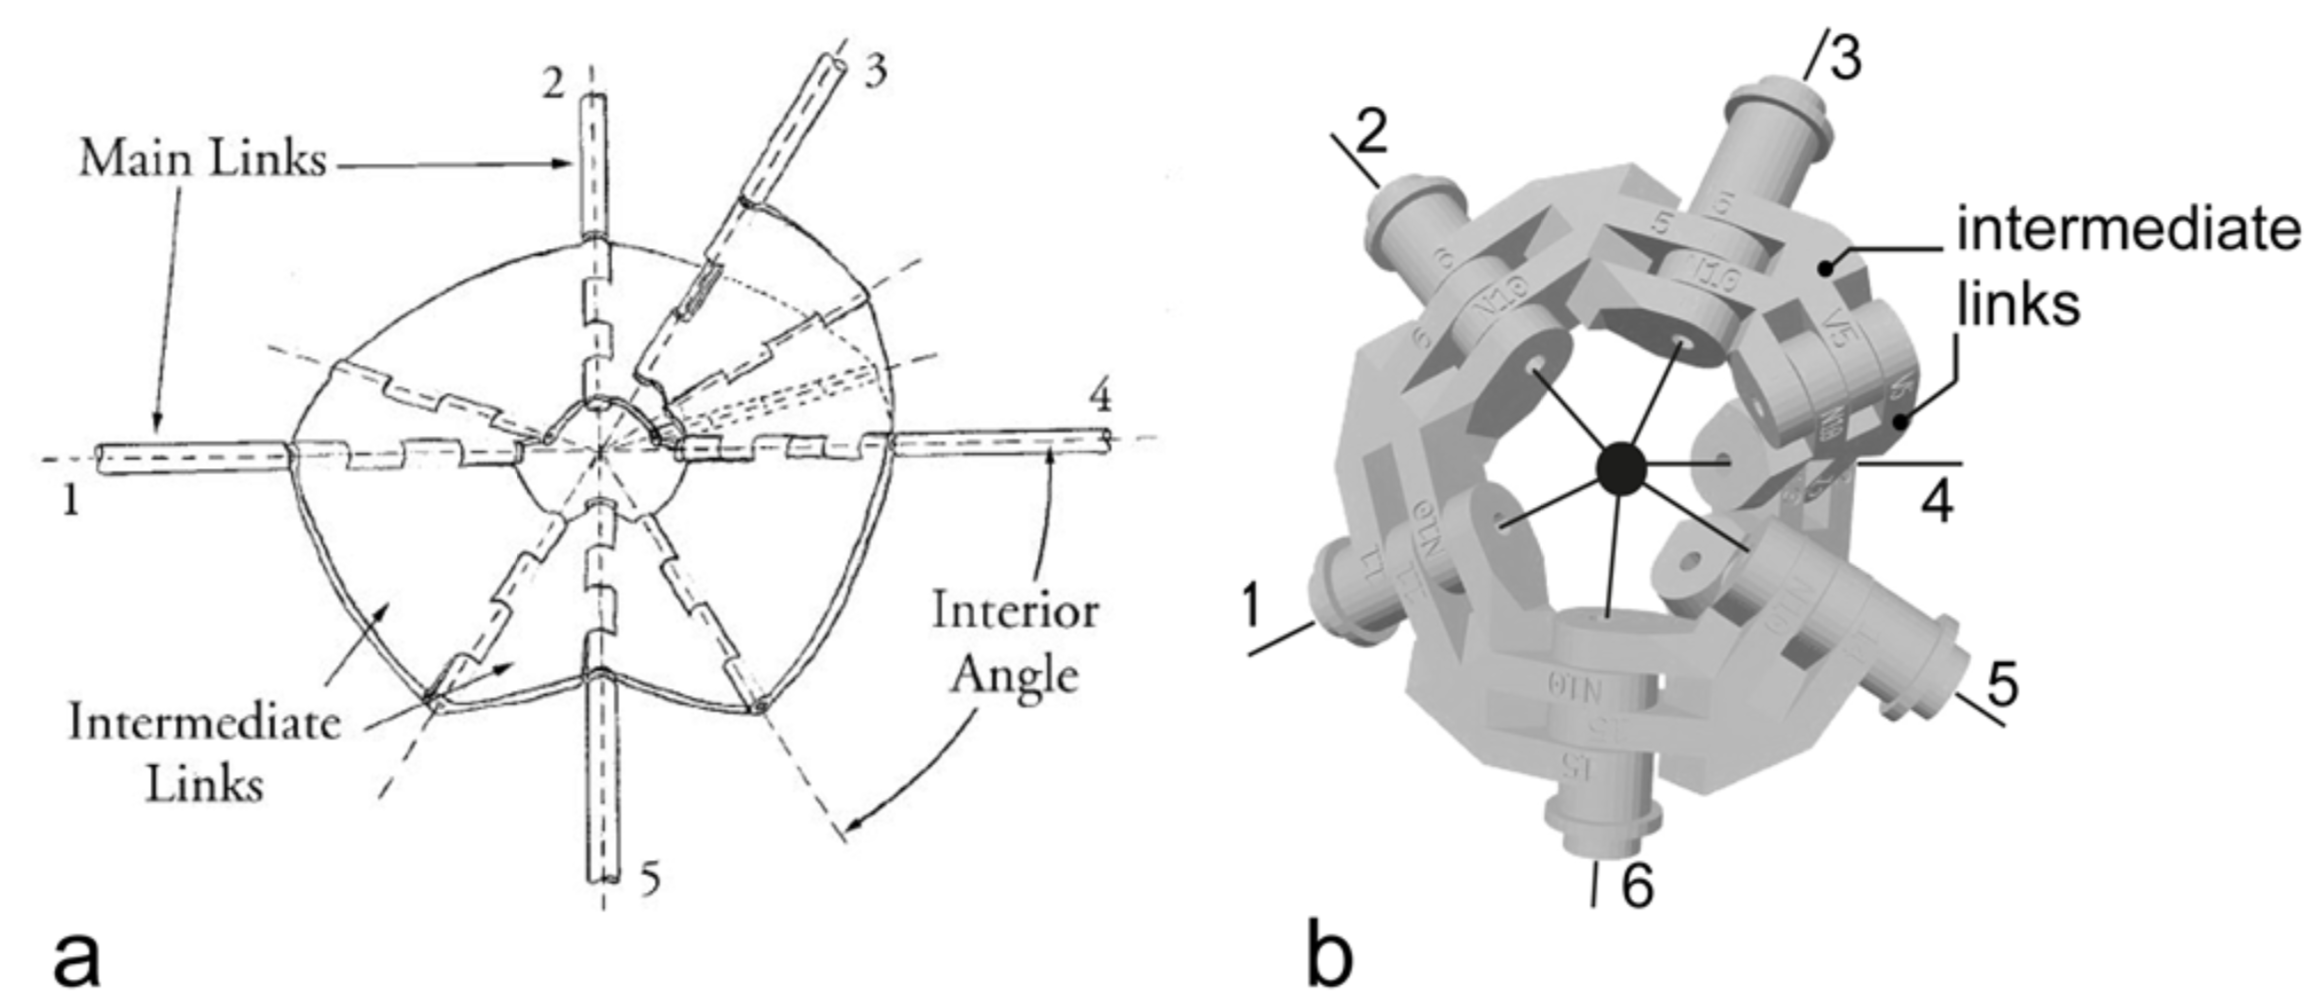
\includegraphics[width=\textwidth]{Hardware/hinge_chain.png}
    \centering
    \caption{(a) spherical joint mechanism connecting 5 links. (b) rendering of TrussFormers' hinge chain design connecting 6 links.}
    \label{fig:hinge_chain}
\end{figure}
We started out using an open hinge chain, meaning that the chain had special end parts which were only connected on one side. This gave us a lot of freedom of movement, however it turned out that this design was not strong enough for our needs and frequently broke during testing builds of the T-Rex. This required us to rethink our design and we came up with a closed hinge chain design.\\
The degrees of freedom (DoF), our hinge system needs to have, underly constraints, allowing us to limit the possible movement of the hinges. The original spherical joint mechanism shown in Figure \ref{fig:hinge_chain}a connected all edges using two hinges, allowing for 2 DoF. This is not necessary if we are dealing with truss structures. An example of TrussFormers's hinge design can be seen in Figure \ref{fig:hinge_chain}b. Only edge 4 is connected to its neighboring edges using two intermediate hinges. All other edges only require rotation (resulting in 1 DoF).\\
The hinge chains are arranged automatically in the structure by our TrussFormer system. This heuristic approach will be described in more detail in Section \ref{sec:hinge_placement_impl}.

\subsubsection{3D printing}
The hubs and connecting cuffs are printed using consumer-grade desktop FDM\footnote{Fused Deposition Modeling} 3D printers. The filament consists of PLA\footnote{Polylactic acid} plastic and the printed objects have a 15\% infill with a wall thickness of 3 mm. We chose PLA filament instead of ABS\footnote{Acrylonitrile butadiene styrene} primarily because it is easier to handle. ABS plastic, while being stronger, needs to be printed on a heated surface, which not many mid-range printers have. As we designed the TrussFormer system for 3D-printing enthusiasts and not professionals, we wanted to target owners of consumer-grade printers. Additionally, PLA consists of organic materials (mainly cornstarch and sugarcane), which makes it biodegradable, as opposed to ABS plastic, which is oil-based.\\
A hub consumes about 50-150g of filament, resulting in a cost of 1-3€.

\section{Actuation}
\begin{figure}[ht!]
    \includegraphics[width=\textwidth]{Hardware/hardware_setup.png}
    \centering
    \caption{Hardware setup for controlling the T-Rex, with Arduino, electric pressure control valves, and compressor.}
    \label{fig:hardware_setup}
\end{figure}
Figure \ref{fig:hardware_setup} shows the main parts of our hardware setup. The electrically controllable pressure regulators receive signals from the control board and limit the air pressure according to the needed level of extension of a given actuator. One pressure regulator is connected to exactly on actuator. The \textit{Airpress HL 360} compressor delivers the regulators with up to 8 bars of pressure.\\
The limited pressure is tunneled to a valve terminal. This terminal opens and closes airflow to the actuators. If it opens a valve, the regulated pressure will enter its air circuit and change the extension of the actuator. If it closes it, the pressure will stay constant and the actuator keeps its position.

\subsection{Electric Actuators}
Early TrussFormer prototypes used electric actuators, instead of the pneumatic ones we used for the T-Rex. Electric actuators can produce a fairly large force and are easier to control, as they can usually provide their current extension. However, at around 0.03 m/s they extend very slowly, compared to our pneumatic actuators, which can reach more than 2 m/s. As our structures are fairly lightweight, the force of the actuators is not a big concern, while the higher speed of pneumatic actuators enables us to create more dynamic structures.

\subsection{Pneumatic Actuators}
We use different kinds of pneumatic actuators, depending on the force needed. Our actuators usually have a piston diameter of 20 - 35 mm and can extend from 40 cm to 80 cm. This length works well with our bottle links, which are 60 cm long, meaning that the middle position of the actuator makes it the same length as the links.\\
A common actuator that could be used is the Festo DSNU round cylinder with a diameter of 32 mm and a hub of 30 cm, as shown in Figure \ref{fig:festo_cylinder}. This cylinder can operate with up to 10 bars, the following values were measured with 6 bars of pressure and at room temperature. Under these circumstances, this actuator can achieve an extension rate of up to 2.3 m/s (without load) with a force of 480N on the extending stroke and 415N on retraction. This force is sufficient for moving the head of our T-Rex up and down, which is the motion requiring the most force in our design. For higher loads, e.g. lifting a human, an actuator with a bigger diameter should be used. A Festo actuator with a diameter of 50 mm is capable of achieving up to 1200 N of force on the extending stroke at 6 bars.
\begin{figure}[ht!]
    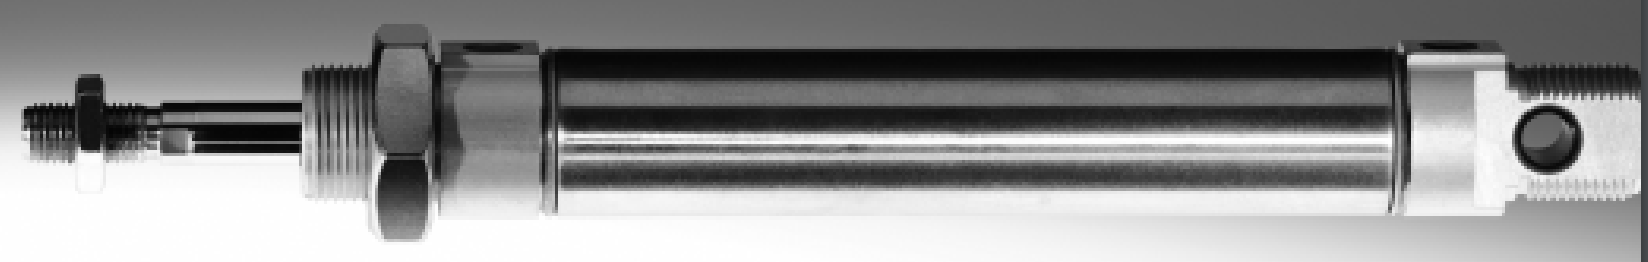
\includegraphics[width=\textwidth]{Hardware/festo_cylinder.png}
    \centering
    \caption{A Festo DSNU cylinder with 32 mm cylinder diameter and 30 cm of hub, as used in our T-Rex.}
    \label{fig:festo_cylinder}
\end{figure}

\section{Control System}
We control the pneumatic actuators using a MIDI control interface. The slider inputs are sent to an Arduino which translates them to control signals for digitally controllable pressure valves. The actuators have two connections for air pipes: one for extending the actuator and one for retracting it. The signal from the slider is interpreted as a mixture between these two inputs, with the slider at the top meaning that all the air is send to the extending input and the slider at the bottom completely retracting it.

\subsection{Valves}
We used two different kinds of valves. \textit{Proportional pressure regulators}, such as the Festo VPPM, are used for open-loop pressure control. Communication to these regulators is achieved with an IO link, which can be connected to a control unit. Digital signals are translated to a proportional opening of the valves, providing a constant and reliable pressure. VPPMs have one input and one output valve. This fact differentiates proportional pressure regulators from \textit{proportional directional control valves}, like the Festo MPYE. These valves have one input, but two outputs, making it possible to connect it to both inputs of a pneumatic actuator. Controlling these valves works similar to proportional pressure regulators and also uses a simple IO link. Digital signals send to this type of valve do not, however, only control the pressure of these outputs, but also the ratio between these two outputs. This makes positional control of actuators possible.

\begin{figure}[ht!]
    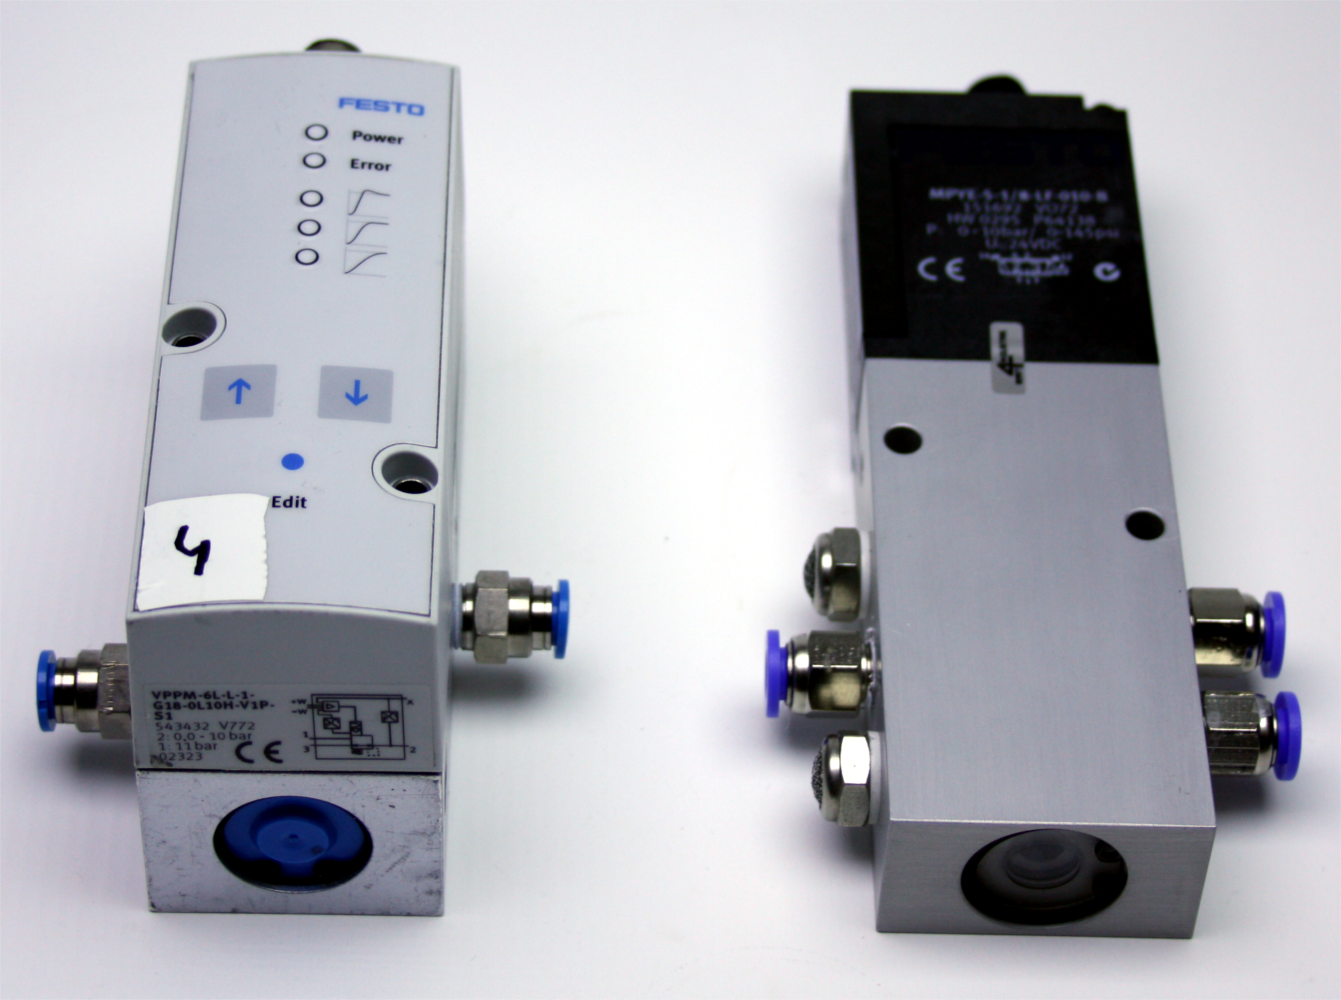
\includegraphics[width=\textwidth]{Hardware/valves.png}
    \centering
    \caption{(left) A proportional pressure regulator with one input and one output. (right) A proportional directional control valve, with one input and two outputs. Both can be attached to an IO link on the top.}
    \label{fig:valves}
\end{figure}

\subsection{Position Sensing}
The MIDI controller is a well working possibility to control actuators. It is, however, an open-loop control, meaning it can not react to external influences, like weight shifts or additional pressure acting on edges. This is not a big problem for our T-Rex example, as it usually moves undisturbed and without external interaction. If we want to create an interactive object, this will not be sufficient.\\
Pneumatic actuators on their own tend to not have the possibility to measure their own rate of extension. We therefore created an easy to build distance sensor, using a string on a spindle. One side of the string is attached to the piston part of the actuator, while the spindle is attached to the static body. While the actuator extends, the spindle will spin, releasing more string. We attached a rotary encoder to the spindle, counting its rotations. Using the diameter of the reel, we can calculate how much string was released during the extension, which correlates to the extension of the piston itself. A prototype of this method can be seen in Figure \ref{fig:position_control}.\\
\begin{figure}[ht!]
    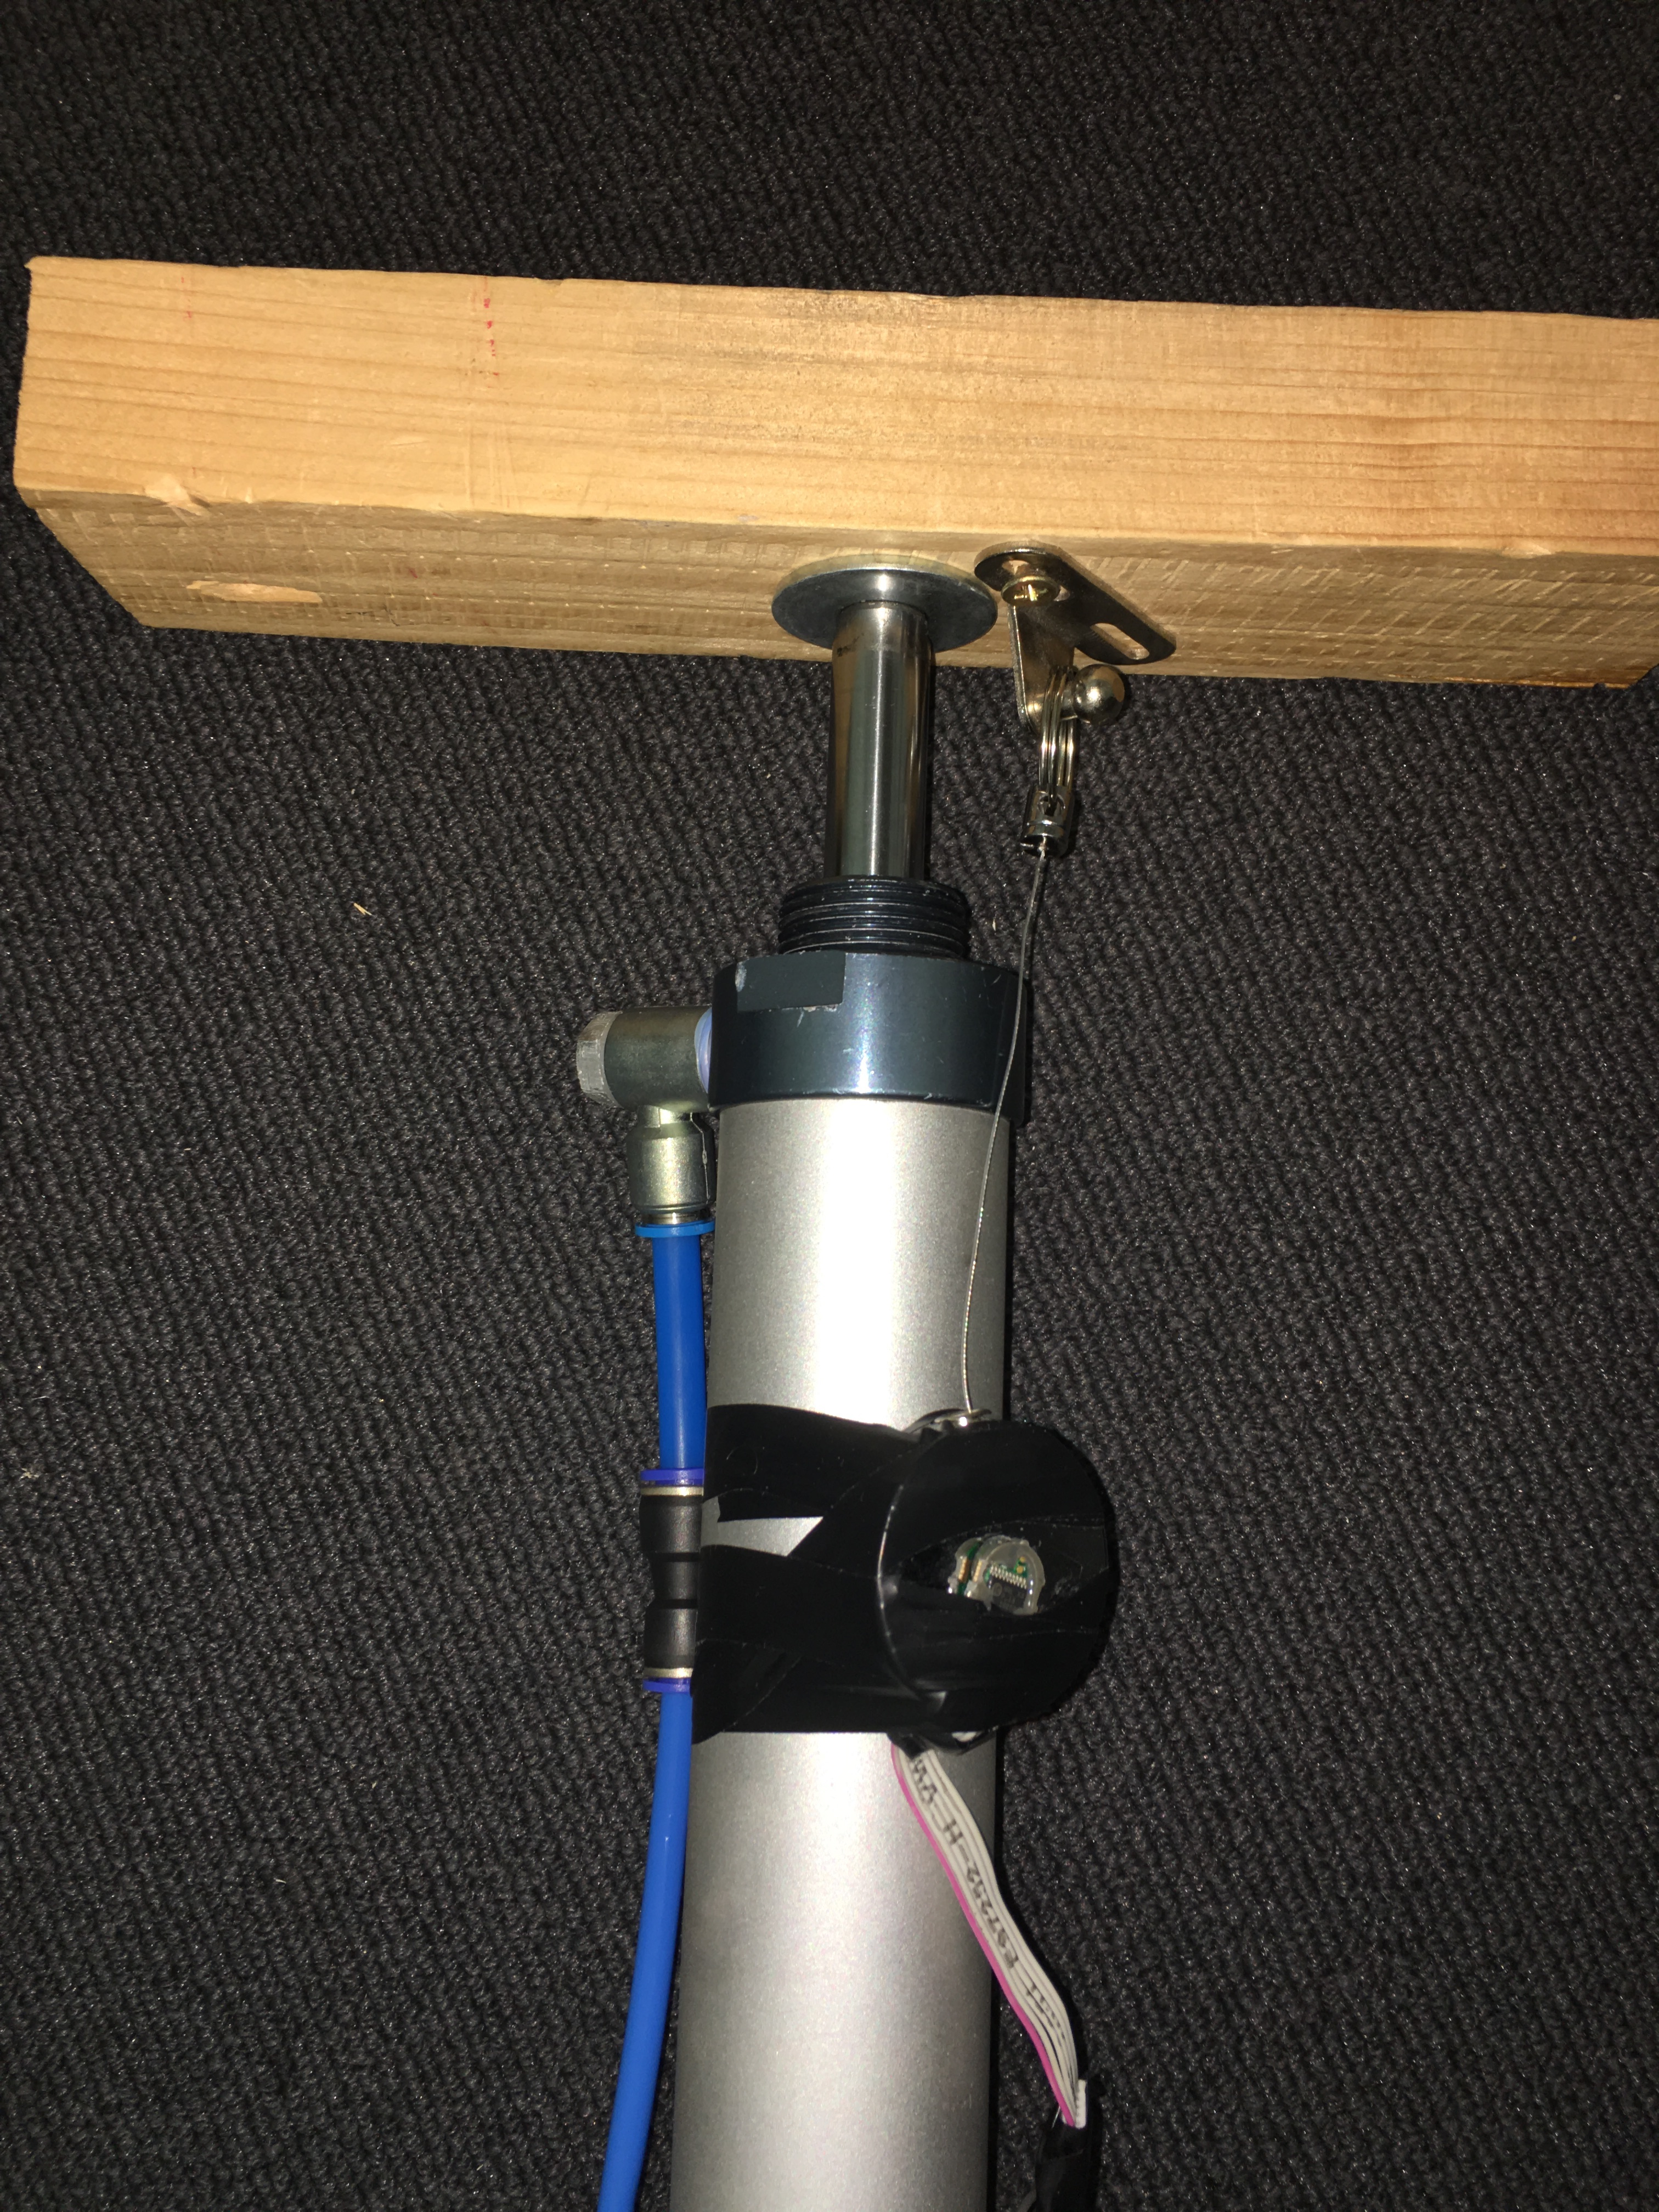
\includegraphics[width=\textwidth]{Hardware/position_controller.png}
    \centering
    \caption{We use a badge holder with a rotary encoder for position sensing. The string of the holder is attached to the actuators body and the extending piston. On extension, the string will roll off the spindle, which we can measure with the encoder and translate into a length.}
    \label{fig:position_control}
\end{figure}
Using this approach, we can have closed-loop control of the actuators, making it possible to constantly monitor its extension and apply force accordingly.

\subsubsection{PID Controller}
We created a rudimentary motion-platform using closed-loop PID control (s.a. Section \ref{sec:pid}). The motion platform has three modes. It starts fully extended, applying a little bit of pressure to keep the actuator upright, but little enough that a human sitting on it pushed it back. If the actuator reached an extension of 10 cm, the control loop applied a holding force, making it possible to sit on the platform without it moving. If the person on the platform applied more force, pushing the piston further down, the third mode activated, which made it oscillate up and down.

\subsection{Control Units}
For our control module we have different approaches for open and closed loop control, as well. Open loop control can be achieved with a simple \textit{Arduino}. It can be attached to a control interface, such as our MIDI controller, and translate the given inputs into signals for the valves.\\
Another logic controller we used is the \textit{Controllino}.
